\documentclass{report}
% Include all project wide packages here.
\usepackage{fullpage}
\usepackage[style=ieee]{biblatex}
\usepackage[dutch]{babel}

\renewcommand{\familydefault}{\sfdefault}

\setmainfont[Ligatures=TeX]{Myriad Pro}
\setmathfont{Asana Math}
\setmonofont{Lucida Console}

\usepackage{titlesec, blindtext, color}
\definecolor{gray75}{gray}{0.75}
\newcommand{\hsp}{\hspace{20pt}}
\titleformat{\chapter}[hang]{\Huge\bfseries}{\thechapter\hsp\textcolor{gray75}{|}\hsp}{0pt}{\Huge\bfseries}
\renewcommand{\familydefault}{\sfdefault}
\renewcommand{\arraystretch}{1.2}
\setlength\parindent{0pt}

%For code listings
\definecolor{black}{rgb}{0,0,0}
\definecolor{browntags}{rgb}{0.65,0.1,0.1}
\definecolor{bluestrings}{rgb}{0,0,1}
\definecolor{graycomments}{rgb}{0.4,0.4,0.4}
\definecolor{redkeywords}{rgb}{1,0,0}
\definecolor{bluekeywords}{rgb}{0.13,0.13,0.8}
\definecolor{greencomments}{rgb}{0,0.5,0}
\definecolor{redstrings}{rgb}{0.9,0,0}
\definecolor{purpleidentifiers}{rgb}{0.01,0,0.01}


\lstdefinestyle{csharp}{
language=[Sharp]C,
showspaces=false,
showtabs=false,
breaklines=true,
showstringspaces=false,
breakatwhitespace=true,
escapeinside={(*@}{@*)},
columns=fullflexible,
commentstyle=\color{greencomments},
keywordstyle=\color{bluekeywords}\bfseries,
stringstyle=\color{redstrings},
identifierstyle=\color{purpleidentifiers},
basicstyle=\ttfamily\small}

\lstdefinestyle{c}{
language=C,
showspaces=false,
showtabs=false,
breaklines=true,
showstringspaces=false,
breakatwhitespace=true,
escapeinside={(*@}{@*)},
columns=fullflexible,
commentstyle=\color{greencomments},
keywordstyle=\color{bluekeywords}\bfseries,
stringstyle=\color{bluestrings},
identifierstyle=\color{purpleidentifiers}
}

\lstdefinestyle{vhdl}{
language=VHDL,
showspaces=false,
showtabs=false,
breaklines=true,
showstringspaces=false,
breakatwhitespace=true,
escapeinside={(*@}{@*)},
columns=fullflexible,
commentstyle=\color{greencomments},
keywordstyle=\color{bluekeywords}\bfseries,
stringstyle=\color{redstrings},
identifierstyle=\color{purpleidentifiers}
}

\lstdefinestyle{xaml}{
language=XML,
showspaces=false,
showtabs=false,
breaklines=true,
showstringspaces=false,
breakatwhitespace=true,
escapeinside={(*@}{@*)},
columns=fullflexible,
commentstyle=\color{greencomments},
keywordstyle=\color{redkeywords},
stringstyle=\color{bluestrings},
tagstyle=\color{browntags},
morestring=[b]",
  morecomment=[s]{<?}{?>},
  morekeywords={xmlns,version,typex:AsyncRecords,x:Arguments,x:Boolean,x:Byte,x:Char,x:Class,x:ClassAttributes,x:ClassModifier,x:Code,x:ConnectionId,x:Decimal,x:Double,x:FactoryMethod,x:FieldModifier,x:Int16,x:Int32,x:Int64,x:Key,x:Members,x:Name,x:Object,x:Property,x:Shared,x:Single,x:String,x:Subclass,x:SynchronousMode,x:TimeSpan,x:TypeArguments,x:Uid,x:Uri,x:XData,Grid.Column,Grid.ColumnSpan,Click,ClipToBounds,Content,DropDownOpened,FontSize,Foreground,Header,Height,HorizontalAlignment,HorizontalContentAlignment,IsCancel,IsDefault,IsEnabled,IsSelected,Margin,MinHeight,MinWidth,Padding,SnapsToDevicePixels,Target,TextWrapping,Title,VerticalAlignment,VerticalContentAlignment,Width,WindowStartupLocation,Binding,Mode,OneWay,xmlns:x}
}

%defaults
\lstset{
basicstyle=\ttfamily\small,
extendedchars=false,
numbers=left,
numberstyle=\ttfamily\tiny,
stepnumber=1,
tabsize=4,
numbersep=5pt
}
\addbibresource{../../library/bibliography.bib}

\title{EPO-2: Niet-lineaire schakelingen - Inleiding}
\author{Luc Does}

\begin{document}

\chapter{Inleiding}
\label{ch:inleiding}

In dit verslag behandelen wij de spanningsgestuurde spanningsdeler m.b.v. een diode als voorbeeld van het gebruik van niet lineaire schakelingen. Deze opdracht sluit aan bij het EPO-2 project en heeft onder meer als doel het gebruik van simulaties te verduidelijken bij de bouw van niet-lineaire schakelingen. \newline
Aangezien de groep is verdeeld in twee delen behandelen wij hier de eerste opdracht om deze uit te leggen aan de andere groep welke de tweede opdracht heeft behandeld. Bij deze uitleg geven wij de uitwerkingen van de opgaves op een verklarende manier.
\newline

\noindent De schakeling van de spanningsdeler is gegeven in de handleiding van de JIT: niet-lineaire schakelingen. Deze geven wij nogmaals in figuur \ref{fig:totaalschema}. Het ingangssignaal wordt gemodelleerd door een wisselspanningsbron van 60Hz met een amplitude van 50mA. De instelspanning V1 en de instelweerstand R1 moeten we in deze opdracht bepalen.

\begin{figure}[H]
	\centering
	\includegraphics[width=0.8\textwidth]{niet-lineaire-schakelingen-schema.pdf}
	\caption{circuit voor spanningsgestuurde spanningsdeler met diode}
	\label{fig:totaalschema}
\end{figure}


\section{1}
Om de diode als een spannings-gestuurde spanningsdeler te gebruiken is het belangrijk om een juiste keuze voor de waardes van $R1$ en $V1$ te maken. Aangezien het analytisch oplossen van niet-lineaire schakelingen zeer lastig is is het gebruik van een simulatieprogramma ideaal om een goede benadering te krijgen van de benodigde waardes. In plaats van de aangewezen Falstad simulator hebben wij gebruik gemaakt van de CircuitLab simulator. Deze simulator is vriendelijker in gebruik terwijl hij wel op het geavanceerdere  Spice is gebaseerd, hierdoor is het voor ons makkelijk om nauwkeurige simulaties uit te voeren.
\newline
De karakteristiek die wij zoeken bij een goed functionerende schakeling is een lineair verband tussen de stroom en de spanning. Bij de waardes $R1 = 1k\Omega$ en $V1 = 1V$ zien we deze karakteristiek terug en daarom hebben we deze gekozen als eerste ruwe waardes.

\section{2}
Bij een groot-signaal circuit gaan we uit van spanningen binnen de schakeling die vele malen groter zijn dan de klein-signalen die de sensor produceert. Hierdoor is dit deel van de schakeling te verwaarlozen, het circuit dat resteert wordt gegeven door \ref{fig:groot}.
We zien dat de wisselspanningsbron is weggevallen aangezien deze een kleinsignaal inhoudt, deze spanningsbron is daarbij een kortsluiting geworden. Ook zien we dat de condensatoren zijn omgevormd tot open klemmen, dit is een gevolg van de afwezigheid van een wisselspanning.
\begin{figure}[H]
	\centering
	\includegraphics[width=0.8\textwidth]{grootsignaal-model.pdf}
	\caption{grootsignaal-model van de schakeling}
	\label{fig:groot}
\end{figure}

\noindent Wanneer we een DC-sweep uitvoeren voor V1 met CircuitLab met betrekking op de stroom door de diode krijgen we de grafiek uit figuur \ref{fig:iv-groot}. Hier valt op te merken dat tot ongeveer 1V een non-lineair verband bestaat tussen de stroom door de diode en de instelspanning. Bij 1.1V kan de spanning verhoogt of verlaagt worden zonder dat het systeem zijn lineariteit verliest. Vandaar dat we 1.1V als instelpunt hebben gebruikt.

\begin{figure}[H]
	\centering
	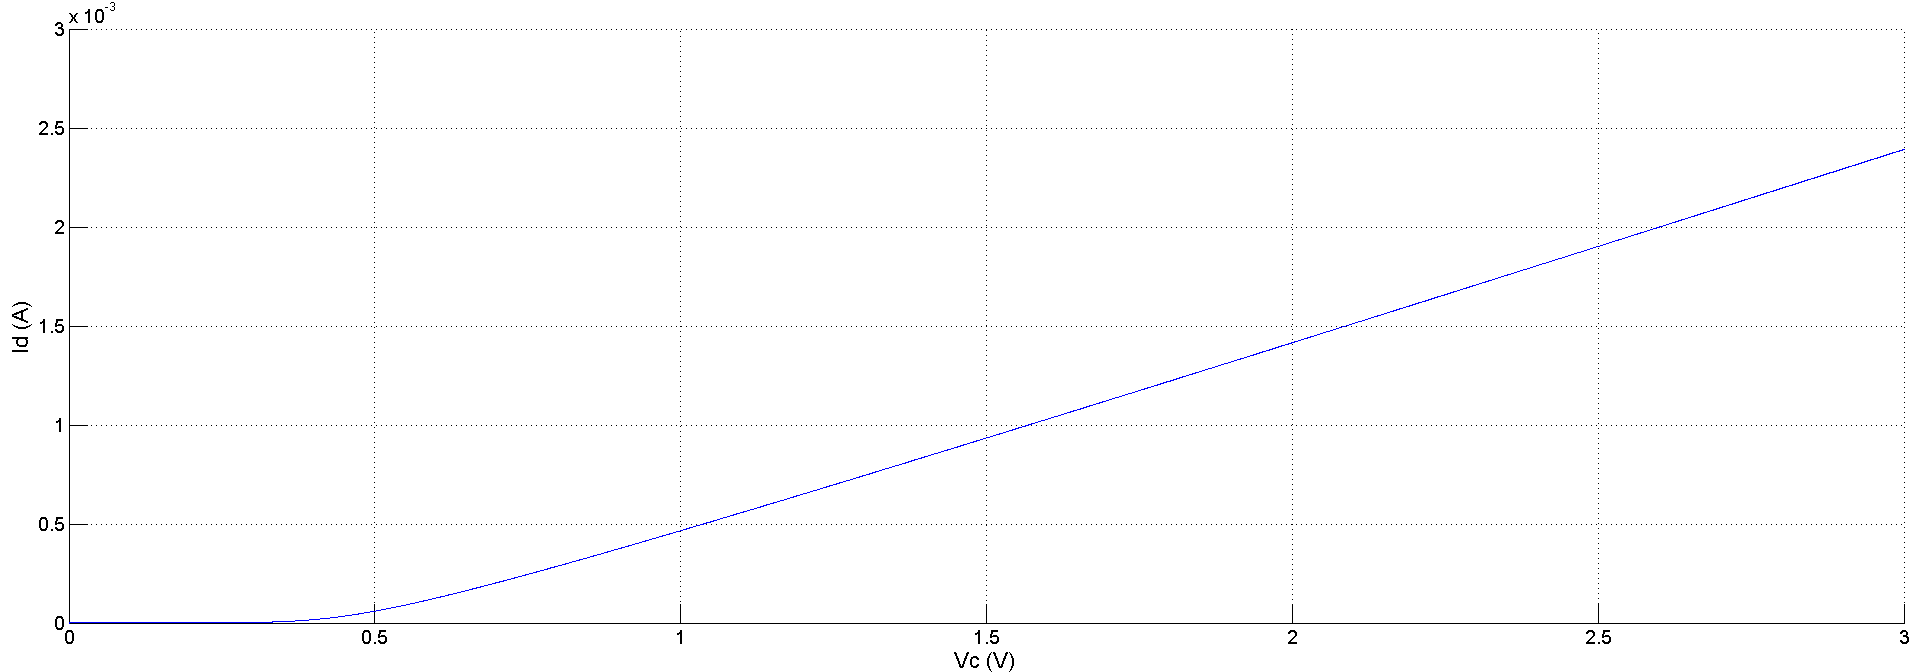
\includegraphics[width=0.8\textwidth]{iv-groot.png}
	\caption{$iv$-karakteristiek van de grootsignaal schakeling}
	\label{fig:iv-groot}
\end{figure}


\section{3}
Met behulp van het CircuitLab voeren wij een DC-sweep uit voor V1. Door de spanning over de diode te delen door de stroom die erdoorheen loopt kunnen wij de differentiële weerstand bepalen. Deze differentiële weerstand staat geplot in figuur \ref{fig:rdv}. Op ons instelpunt van 1.1V bedraagt de differentiële weerstand $971.4k\Omega$
\begin{figure}[H] 
	\centering
	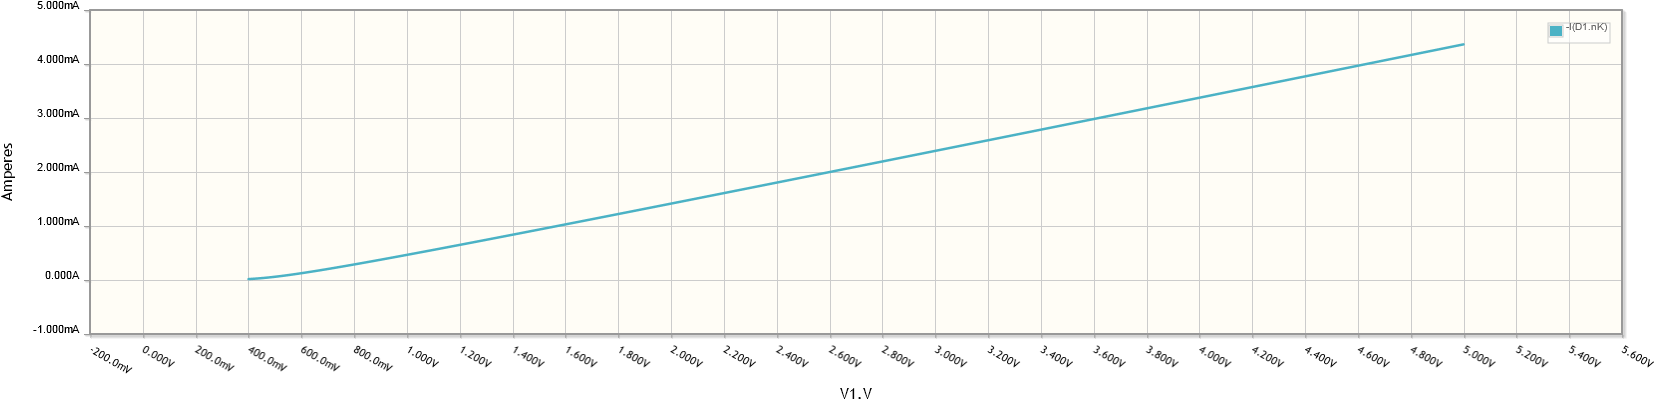
\includegraphics[width=0.8\textwidth]{iv.png}
	\caption{$iv$-karakteristiek van de schakeling}
	\label{fig:iv}
\end{figure}

\begin{figure}[H]
	\centering
	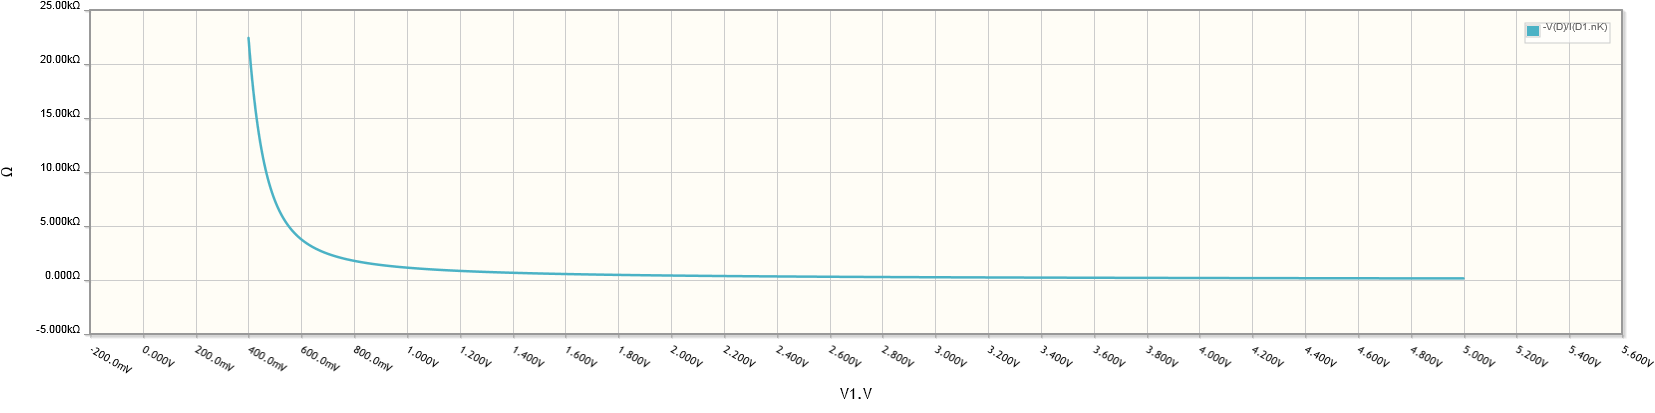
\includegraphics[width=0.8\textwidth]{RdV.png}
	\caption{$r_dv$-karakteristiek van de schakeling}
	\label{fig:rdv}
\end{figure}

\end{document}